\documentclass[polish,a4paper]{article}
\usepackage[utf8]{inputenc}
\usepackage[T1]{fontenc}
%%\usepackage{polski}
\usepackage{amsmath}
\usepackage{amssymb,amsfonts,amsthm}
\usepackage{babel}
\usepackage{hyperref}
\usepackage{xcolor}
\usepackage{graphicx} 
\usepackage{caption}
\usepackage{subcaption}
\usepackage{listings}
\usepackage{anysize}
%%\usepackage{tabto}

\graphicspath{ {img/} }
\marginsize{2.5cm}{2.5cm}{0cm}{3cm}

\definecolor{codegreen}{rgb}{0,0.6,0}
\definecolor{codegray}{rgb}{0.5,0.5,0.5}
\definecolor{codepurple}{rgb}{0.58,0,0.82}
\definecolor{backcolour}{rgb}{0.95,0.95,0.92}

\lstdefinestyle{mystyle}{
	backgroundcolor=\color{backcolour},   
	commentstyle=\color{codegreen},
	keywordstyle=\color{magenta},
	numberstyle=\tiny\color{codegray},
	stringstyle=\color{codepurple},
	basicstyle=\ttfamily\footnotesize,
	breakatwhitespace=false,         
	breaklines=true,                 
	captionpos=b,                    
	keepspaces=true,                 
	numbers=left,                    
	numbersep=5pt,                  
	showspaces=false,                
	showstringspaces=false,
	showtabs=false,                  
	tabsize=2
}

\lstset{style=mystyle}

\begin{document}
	\begin{center}
		\begin{tabular}{ p{0.32\textwidth} p{0.15\textwidth} p{0.15\textwidth} p{0.12\textwidth} p{0.12\textwidth} }
			
			&   &   &   &  \\
			\hline
			\multicolumn{5}{|c|}{}\\[-1ex]
			\multicolumn{5}{|c|}{{\LARGE \textbf{Laboratorium z przedmiotu Systemy wbudowane (SW)}}}\\
			\multicolumn{5}{|c|}{}\\[-1ex]
			\hline
			\hline
			
			\multicolumn{5}{|c|}{}\\[-1ex]
			\multicolumn{5}{|c|}{{\LARGE Zadanie nr 3}}\\
			\multicolumn{5}{|c|}{}\\[-1ex]
			\hline
			\hline
			
			\multicolumn{5}{|c|}{}\\[-1ex]
			\multicolumn{5}{|c|}{{\textbf{Temat zajęć:} Arduino – elementy wykonawcze}}\\
			\multicolumn{5}{|c|}{}\\[-1ex]
			\hline
			\hline
			
			\multicolumn{1}{|l|}{Prowadzący} &
			\multicolumn{2}{|l|}{Autorzy} &
			\multicolumn{1}{|l|}{Grupa dziekańska:}
			&
			\multicolumn{1}{|l|}{I1.2} \\
			\multicolumn{1}{|c|}{mgr inż. Ariel Antonowicz} &
			\multicolumn{2}{|c|}{148088 i 148121} &
			\multicolumn{1}{|c|}{\textbf{Ocena:}} &
			\multicolumn{1}{|c|}{}\\
			\hline
			\hline
		\end{tabular}
	\end{center}
	
	\section{Wyświetlacz LCD + I2C}
	\begin{figure}[h!]
		\begin{center}
			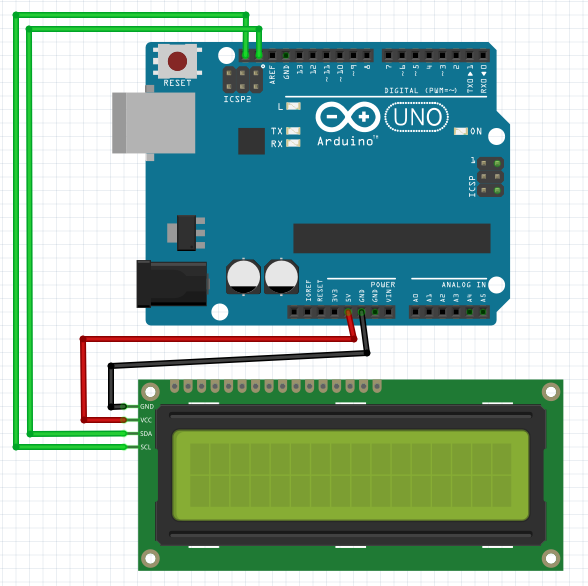
\includegraphics[scale=0.42]{01_hello_world_i2c.png}
			\caption*{Schemat podłączenia wyświetlacza do Arduino}
		\end{center}
	\end{figure}
	\begin{figure}[h!]
		\begin{lstlisting}[language=C++]
			#include <LiquidCrystal_I2C.h>
			LiquidCrystal_I2C lcd(0x27,16,2);
			
			void setup() {
				lcd.init();
				lcd.clear();
				lcd.backlight();
				
				lcd.setCursor(2,0);
				lcd.print("Hello World");
			}
			
			void loop() {}
		\end{lstlisting}
		\caption*{Kod użyty do wyświetlenia "Hello World'a"}
	\end{figure}
	
	\newpage
	
	\section{Serwomechanizm}
	\begin{figure}[h!]
		\begin{center}
			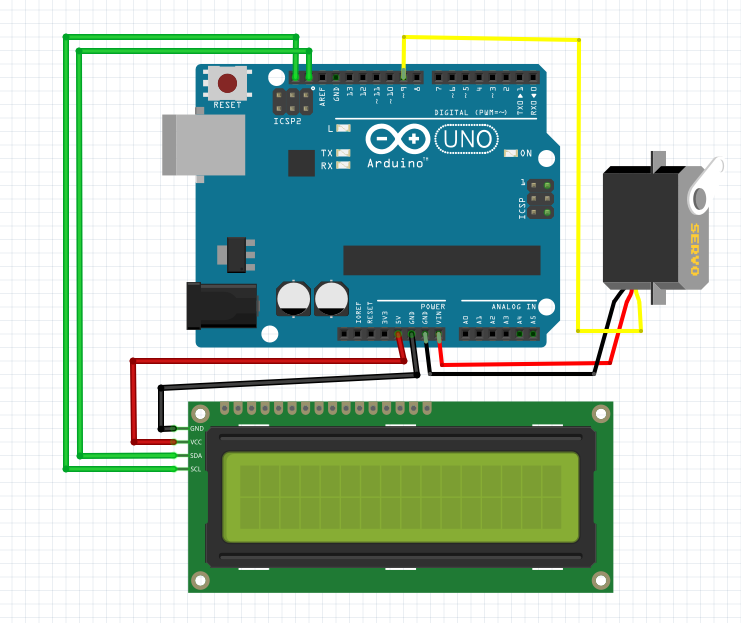
\includegraphics[scale=0.35]{02_servo.png}
			\caption*{Schemat podłączenia servomotor'a do Arduino}
		\end{center}
	\end{figure}
	\begin{figure}[h!]
		\begin{lstlisting}[language=C++, basicstyle=\tiny]
			#include <LiquidCrystal_I2C.h>
			#include <Servo.h>
			LiquidCrystal_I2C lcd(0x27,16,2);
			Servo myservo;
			int pos = 0;
			bool state = true; // true - zamkniete drzwi	
			void setup() {
				Serial.begin(9600);
				myservo.attach(9);
				myservo.write(0);
				lcd.init();
				lcd.clear();
				lcd.backlight();
			}
			void loop() {
				while (Serial.available() == 0) {}
				String op = Serial.readString();  //read until timeout
				op.trim();                        // remove any \r \n whitespace at the end of the String
				if (op == "o" && state) {
					lcd.clear();
					lcd.setCursor(0,0);
					lcd.print("Drzwi sie");
					lcd.setCursor(0,1);
					lcd.print("Otwieraja");
					state = false;
					for(pos = 0; pos <= 180; pos += 1) // obrot od 0 do 180 stopni
					{                                  
						myservo.write(pos);     
						delay(15);                       
					}
					lcd.clear();
				} else if (op == "z" && !state) {
					lcd.clear();
					lcd.setCursor(0,0);
					lcd.print("Drzwi sie");
					lcd.setCursor(0,1);
					lcd.print("Zamykaja");
					state = true;
					for(pos = 180; pos>=0; pos-=1) // obrot od 180 do 0 stopni
					{
						myservo.write(pos);              
						delay(15);                       
					}
					lcd.clear();
				} else if (op == "z" && state){
					lcd.clear();
					lcd.setCursor(0,0);
					lcd.print("Drzwi juz sa");
					lcd.setCursor(0,1);
					lcd.print("Zamkniete");
				} else if (op == "o" && !state){
					lcd.clear();
					lcd.setCursor(0,0);
					lcd.print("Drzwi juz sa");
					lcd.setCursor(0,1);
					lcd.print("Otwarte");
					delay(15*180);
				} else{
					lcd.clear();
					lcd.setCursor(0,0);
					lcd.print("Niepoprawna");
					lcd.setCursor(0,1);
					lcd.print("Operacja");
					delay(15*180);
				}
			}
		\end{lstlisting}
		\caption*{Kod użyty do zadania "otwieranie drzwi"}
	\end{figure}
	
	\newpage
	
	\section*{Źródła}
	\begin{enumerate}
		\item \href{https://forum.fritzing.org/t/16x2-i2c-lcd-part/2041/4}{Fritzing}
		\item Materiały podane przez prowadzącego na platformie ekursy.
		\item \href{https://create.arduino.cc/projecthub/jehankandt/arduino-16x2-lcd-display-with-i2c-hello-world-4b1a41}{create.arduino.cc}
		\item \href{http://akademia.nettigo.pl/serwomechanizm/}{akademia.nettigo.pl} 
	\end{enumerate}
	\begingroup
	\hypersetup{hidelinks}
	\tableofcontents
	\endgroup
\end{document}
